\documentclass[tikz,border=2pt]{standalone}
\renewcommand{\familydefault}{\sfdefault}
\usetikzlibrary{arrows.meta,calc,positioning}
\tikzset{every picture/.style={line width=1pt, >=Stealth},
         hl/.style={fill=black, fill opacity=0.12, text opacity=1}}
\begin{document}
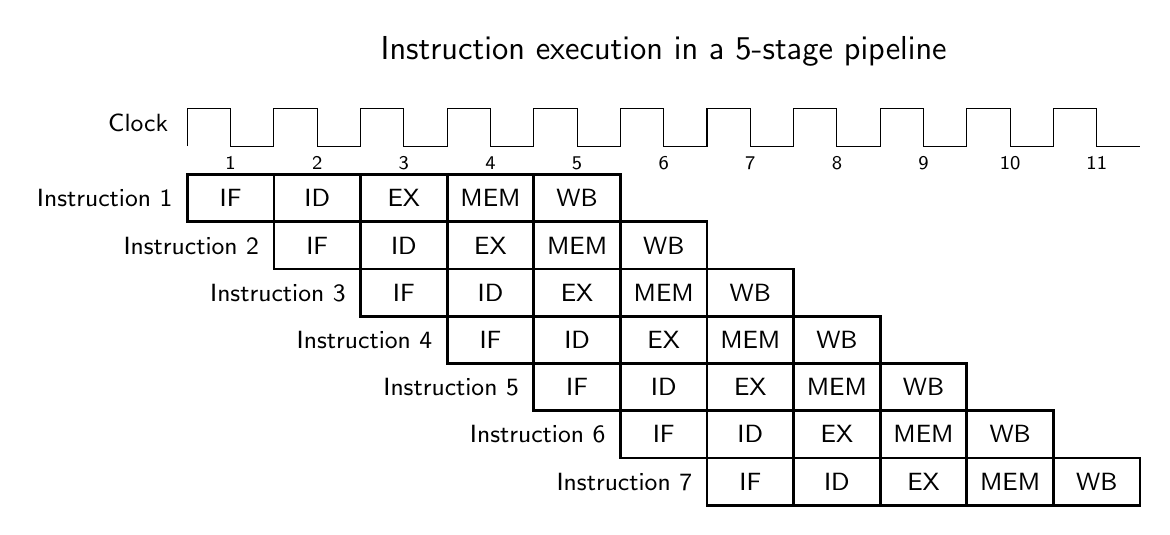
\begin{tikzpicture}[x=1.1cm, y=0.6cm, cell/.style={draw, minimum width=1.1cm, minimum height=0.6cm, font=\small}]
  % \pipe{row}{first cycle}{stage/style, ...}: one instruction, one cell per clock cycle
  \newcommand{\pipe}[3]{\foreach \v/\s [count=\i from 0] in {#3} \node[cell, \s] at (#2 + \i, -#1) {\v};}
  \node[font=\large] at (5, 2.6) {Instruction execution in a 5-stage pipeline};
  % One clock pulse per cycle; a new instruction enters the pipeline every cycle.
  \node[left, font=\small, align=right] at (-0.6, 1.1) {Clock};
  \draw[thin] (-0.5, 0.6) \foreach \t in {0, ..., 10} {-- (\t - 0.5, 0.6) -- (\t - 0.5, 1.4) -- (\t, 1.4) -- (\t, 0.6)} -- (10.5, 0.6);
  \foreach \t in {1, ..., 11} \node[font=\scriptsize] at (\t - 1, 0.25) {\t};
  \foreach \k in {1, ..., 7} {
    \node[left, font=\small] at (\k - 1.55, -\k + 0.5) {Instruction \k};
    \pgfmathsetmacro{\row}{\k - 0.5}
    \pipe{\row}{\k - 1}{IF/, ID/, EX/, MEM/, WB/}
  }
\end{tikzpicture}
\end{document}
